\documentclass[10pt]{jarticle}
\usepackage{float}
\usepackage{adrobo_abst}
\usepackage[dvipdfmx]{graphicx}
\usepackage{amssymb,amsmath}
\usepackage{bm}
\usepackage[superscript]{cite}
\usepackage{enumerate}
\usepackage{url}
%\usepackage[absolute]{textpos}

\renewcommand\citeform[1]{(#1)}

\begin{document}
    
    \makeatletter
    \doctype{2023年度卒業論文概要}
    \title{画像認識を用いた自動打刻の勤怠管理システム}{}
    \etitle{Attendance management system using image recognition}{}
    
    \author{19C1004\hspace{.5zw}池田泉海}
    \eauthor{Motomi Ikeda}
    
    \makeatother
    
    \abstract{
    We propose an automated attendance management system using image recognition.
    Conventional attendance management systems require manual time stamping.
    This leads to problems such as the effort involved in stamping for each entry and exit.
    Additionally, there is a possibility of forgetting to stamp.
    To avoid this problem, we attempt to use image recognition to automate the time stamping process.
    The proposed method detects attendance and departure by employing image recognition to detect each person.
    As the result of experiments, 
    we confirmed that the system we built can automatically perform the procedure from person detection to data uploading to the application.
    }
    
    \keywords{Attendance management system, Automated time stamping, Real-time object detection}
    
    \maketitle
    
    \supervisor{指導教員:上田隆一~准教授}
    
    \section{緒\hspace{2zw}言}%===========================
近年,労働環境の変化に伴い,効率的で正確な勤怠管理の重要性が増している.
そのため、勤怠管理システムでは,打刻に生態認証や顔認証を導入するなどして,
データの客観性が高められている.
しかし,ほとんどの勤怠管理システムは手動での打刻が必要であり,
手動打刻には出退勤毎の打刻労力や打刻忘れ等の問題が存在する.\par
本研究では,これらの問題に対処するためにYOLOv8\cite{Ultralitics}による画像認識で打刻を自動化した勤怠管理システムを提案する.
YOLOv8は物体検出アルゴリズムの一つで,
リアルタイムでの物体検出によく用いられている.
これはYOLOが画像を一度だけ見て物体の位置とクラスを同時に予測することで
高速な物体検出ができるためである.\par
これらの特徴を利用して,リアルタイムでカメラ画像から人物を検出し、それらのタイミングを打刻とすることで打刻を自動化する.
打刻を自動化することで,従来の手動で打刻をする手法に比べ,利用者にとって手間を軽減し,打刻忘れを防止することができると考えられる.

    \section{構築するシステム}%===========================
本研究では、図\ref{configuration}に示した構成で勤怠管理システムを作成する。
システムの詳細について次項、次々項で説明する。

\begin{figure}[!h]
\centering
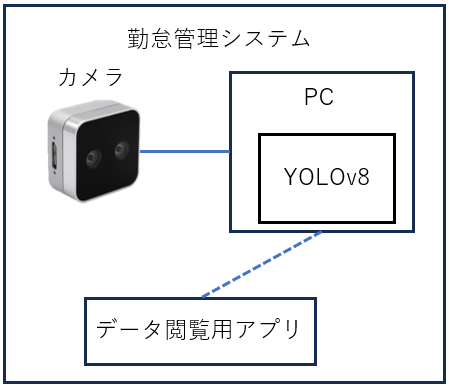
\includegraphics[width=0.8\linewidth]{fig/system.png}
\caption{System configuration}
\label{configuration}
\end{figure}

    \subsection{入退室する人物の検出}
設置されたカメラを指定した時間だけ起動しておき、カメラ映像を約0.2秒毎に画像で取得する。
取得した画像からYOLOv8を用いて人物を検出する。
画像から人物が検出された場合のみ画像を保存する。
その日保存された最初の画像と最後の画像が保存された時間をそれぞれ出勤時間、
退勤時間とする。

    \subsection{データのアップロード}
データ閲覧用のwebアプリに出退勤時の画像データと日時データをアップロードする。
毎日指定した時間になると、その日に保存されたデータが自動でアプリにアップロードされる。


     
    \section{実験}%===========================
実機を用いて図\ref{configuration}のシステムを構築し、
人物の検出からデータのアップロードまで動作可能か検証する。
検証に使用するカメラはIntel Realsense Depth Camera D405\cite{camera}、
PCはWindows10でRAMが32GBのものを用いる。

    \subsection{入退室する人物の検出}
        \label{experiment1}
% 部屋の出入り口にカメラを設置し、入退室する人物が検出できるか実験を行った。

入退室時に人物が検出できるか実験する。
部屋の出入り口にカメラを設置する。
人物検出のモデルを指定した時間の間動かしておき、常に人物の検出を行う。
人物が検出された際は、その画像を保存する。
% 人物検出と保存までできているかの実験

図\ref{Image acquisition}から、カメラからの映像を約0.2秒毎に画像で取得できていることがわかる。
また、図\ref{person detection}から人物が画像内に写った場合、人物検出ができていることがわかる。

\begin{figure}[!h]
    \centering
    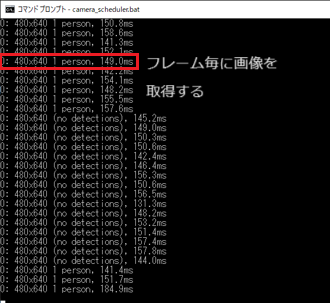
\includegraphics[width=0.8\linewidth]{fig/frame2.png}
    \caption{Image acquisition}
    \label{Image acquisition}
    \end{figure}

\begin{figure}[!h]
    \centering
    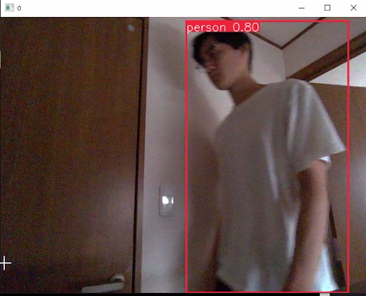
\includegraphics[width=0.8\linewidth]{fig/boundingbox.png}
    \caption{person detection}
    \label{person detection}
    \end{figure}

    \subsection{検出可能な歩行速度}
    入退室時のカメラ前を通る速度を上げた場合にも人物の検出が可能か実験する。
    3つの速度について実験を行った。
    一般的な歩行速度の1.3~m/s、早歩きの速度の1.9~m/s、走る速度の2.2~m/sでの入退室をそれぞれ10回繰り返し、人物検出ができるか確認した。 
    実験の結果、すべての入退室で人物を検出することができた。


    \subsection{データのアップロード}
% 人物を検出した際に保存された画像データと日時データを
% 指定した時間に自動でアプリ上にアプロードをすることができるか実験する。
% 図3のように、アプリ上でデータを確認することができ、データがアップロードできていることが分かる。

指定した時間に自動でアプリ上にデータをアップロードすることができるか実験する。
3・1節で保存された画像データから、
出退勤時の画像とそれに紐づく日時データを取り出す。
指定した時間にアプリへHTTPリクエストを送り、
取り出したデータをデータベースに保存する。
画像を取り出してアプリにリクエストを送るプログラムを、指定した時間に実行することで、
自動アップロードを実現する。
プログラムを実行した結果、図\ref{application}のように、アプリ上でデータを確認することができ、データがアップロードできていることがわかる。
\begin{figure}[!h]
    \centering
    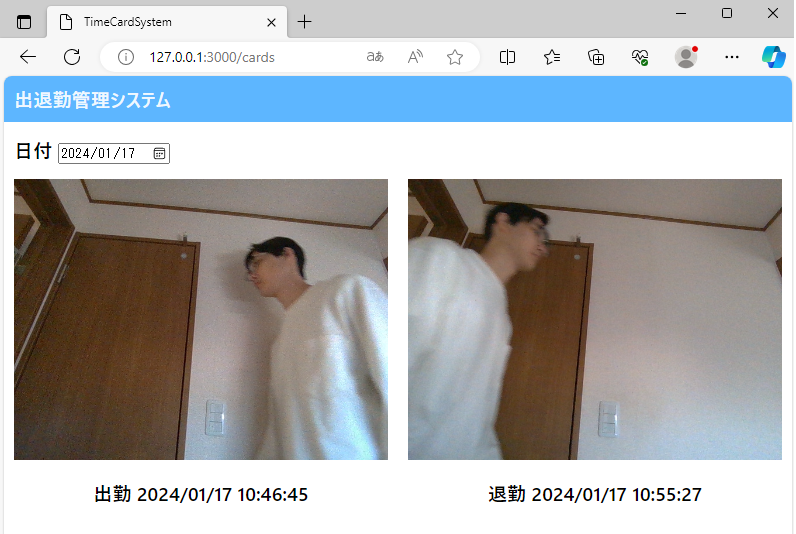
\includegraphics[width=1.0\linewidth]{fig/application3.png}
    \caption{management application}
    \label{application}
    \end{figure}

    \section{結\hspace{2zw}言}%===========================
本研究では、YOLOv8で人物検出をすることで、
画像認識を用いた自動打刻の勤怠管理システムを提案した。
実験より、人物検出からアプリへのデータのアップロードまでを自動的に行うシステムが動作可能なことを確認した。

% もう少し書く
    \vspace{5truemm}
    {\footnotesize
        \begin{thebibliography}{99}

            \bibitem{Ultralitics}
            Ultralytics YOLOv8: 
            \url{https://github.com/ultralytics/ultralytics}, 
            (参照日 2023年12月17日).

            \bibitem{camera}
            Intel Realsense Depth Camera D405: 
            \url{https://www.intelrealsense.com/depth-camera-d405/}, 
            (参照日 2023年12月17日).

        \end{thebibliography}
    }
    \normalsize

\end{document}
